\documentclass[a4paper]{article}
\usepackage[utf8]{inputenc}
\usepackage{erk}
\usepackage{times}
\usepackage{graphicx}
\usepackage{subcaption}
\usepackage{tikz}
\usepackage{amsmath}
\usetikzlibrary{positioning}
\graphicspath{{Images/}}
\usepackage[top=22.5mm, bottom=22.5mm, left=22.5mm, right=22.5mm]{geometry}

\usepackage{cuted}
\usepackage{multirow}
\usepackage{makecell}

\usepackage[slovene,english]{babel}



% local definitions
\def\footnotemark{}%  to avoid footnote on cover page

\begin{document}
%make title
\title{Uporaba spodbujevanega učenja s povratno arhitekturo GRU za kompleksne gibe dvokolesnega mobilnega robota}
\author{Jaka Verk$$} 
\affiliation{$$University of Maribor, Faculty of Electrical Engineering and Computer Science\\ 
$$Koroška cesta 46, 2000 Maribor, Slovenia  }

\email{E-pošta: jaka.verk@student.um.si}

\maketitle

%\thispagestyle{empty}

\begin{abstract}{Reinforcement Learning with a Recurrent Architecture GRU for Complex Movements of a Two-Wheeled Mobile Robot}
Two-wheeled robots capable of balancing on a single wheel present a substantially harder control problem than conventional two-wheel balancing, with no closed-form model for the tilted equilibrium. This paper presents, to the best of our knowledge, the first reinforcement learning based controller for sustaining a two-wheeled robot in a stable single-wheel stance, trained end-to-end with PPO using a compact Gated Recurrent Unit (GRU) architecture that implicitly encodes system dynamics through its hidden state. The network is sized for real-time deployment on an STM32F446RE microcontroller at 50 Hz; domain randomization and a three-stage roll-perturbation curriculum bridge the sim-to-real gap. The learned policy proves capable of achieving and maintaining balance across a wide range of initial roll angles, reaching near-100\% survival probability within the trained $\pm 11°$ band around the 47° equilibrium stance.

%This paper investigates the use of deep reinforcement learning to solve the complex balancing problem of a wheeled-legged robot on a single wheel. This task represents a highly unstable, coupled, and underactuated control challenge, where pitch is managed via the drive wheel and roll is controlled through the leg joints. We utilize the Proximal Policy Optimization (PPO) algorithm within a physics simulation to train a robust control policy without requiring an explicit analytical model of the system's dynamics. Key features of our approach include a multi-phase learning curriculum to gradually broaden the range of starting conditions, and a reward function designed to let the agent autonomously discover its equilibrium roll angle rather than having it pre-defined. To bridge the Sim2Real gap, the solution incorporates domain randomization and is optimized for deployment on low-power embedded hardware, specifically an STM32F446RE microcontroller. Experimental results in simulation demonstrate a survival probability of 99.5\% at the optimal roll angle, confirming that the trained policy effectively masters the robot's inherent instability and successfully identifies its balance point.
\end{abstract}


\selectlanguage{slovene}


  
%Poglavja
  
%Uvod
\section{Uvod}

Mobilni roboti, namenjeni za uporabo v nestrukturiranem naravnem okolju - gozdovi, gradbišča in področja naravnih nesreč, se pogosto poslužujejo uporabe koles v kombinaciji z kontroliranimi nogami, kjer žrtvujejo energijsko učinkovitost lažjemu prilagajanju terenu. Zadnje raziskave so prikazale, da se takšni kolesno-roboti lahko prilagajajo zahtevnemu okolju in imajo sposobnosti premagovanja ovir, vožnje po naklonini in zanesljivo delujejo v skrajnih okoljih, kot so gorske planote \cite{Wang2025Whee}.
  Krmilne strategije, ki poganjajo takšne robote so skoraj brez izjem učene s pomočjo spodbujevanega učenja (angl. RL, reinforcement learning), omogočeno s pomočjo GPU-po\-spe\-še\-nim izvajanjem več tisoč instanc fizikalnih simulacij na enkrat. V \cite{Rudin2022Lear} so pokazali, da lahko množično vzporedno učenje v kombinaciji z večfaznim učenjem na\-ra\-šča\-jo\-če težavnosti terena in motenj v nekaj minutah ustvari robustne politike hoje štirinožnih robotov ter da se politike, naučene izključno v simulaciji, brez dodatnega prilagajanja lahko neposredno prenesejo na fizično strojno opremo.
  
  Nadaljnje raziskave so se posvetile ugotovitvam, katere arhitekture so najboljše za uporabo kot strategijo v RL \cite{Smirnov2025RLBe}. Primerjali so usmerjene, povratne (LSTM, GRU), transformerske in arhitekture s prostorom stanj (Mamba) na podlagi različnih nalog krmiljenja z RL ter ugotovili, da so pri nalogah, ki zahtevajo vzpostavljanje ravnotežja in stabilnosti pod delnim opazovanjem stanj, pri omejeni strojni opremi najboljša izbira povratne arhitekture kot sta GRU (angl. gated recurrent unit) in LSTM (angl. long short term memory).

  V sorodnem delu \cite{Tofant2025Dife} so zasnovali agilnega dvokolesnega robota z zaprto kinematično verigo petih členov, pri čemer nogi vsake strani poganjata dva motorja in kolesi neposredno gnana motorja. Stabilizacijo nagiba robota so dosegli s kaskadnim regulatorjem sestavljenim iz notranje zanke, ki uporablja kvadratični integralni regulator (LQI) in zunanje zanke, poslužejoče se PID. Pristop eksplicitno ne uporablja globokega učenja pri čemer robot v vseh manevrih ravnotežje ohranja na obeh kolesih hkrati.
  
  V tem delu za dvokolesnega robota iz \cite{Tofant2025Dife} uvedemo krmilno strategijo, ki vzdržuje trajno, statično pozo na enem samem kolesu, stanje bistveno zahtevnejše od dvokolesnega ravnotežja. S tem, kolikor nam je znano, predstavljamo prvo naučeno strategijo za ohranjanje ravnotežja dvokolesnega robota na enem kolesu.
  
  Za reševanje obravnavane naloge ravnotežja smo predhodno preizkusili standardno usmerjeno nevronsko mrežo (angl. MLP, multilayer perceptron), vendar se je ta v prisotnosti senzornega šuma in časovnih zakasnitev izkazala za nestabilno ter ni konvergirala k zanesljivemu ravnotežju. Ti rezultati se skladajo z ugotovitvami študije \cite{Smirnov2025RLBe}, kjer avtorji ugotavljajo, da MLP mreže sicer omogočajo visoko učinkovitost, v okoljih z delno opazljivostjo pa odpovedo, zato smo kot osnovo strategije uporabili arhitekturo GRU z nevronsko mre\-žo, ki ji ni treba poznati niti eksplicitnega modela dinamike niti njegovih parametrov za posamezno konfiguracijo nog, s čimer nadaljujemo v smeri nadaljnjega dela, ki ga predlagajo avtorji \cite{Tofant2025Dife}.
  V nasprotju z GRU arhitekturami, primerjanimi v \cite{Smirnov2025RLBe} zgolj v simulacijskih okoljih, je naša povratna politika načrtovana in naučena za dejansko namestitev na vgrajenem mikrokrmilniku (STM32) pri nadzorni frekvenci 50 Hz, kar zahteva izjemno majhno strategijo za namen prenosljivosti strategije iz simulacijskega okolja v resnično, računsko omejeno strojno opremo za razliko od \cite{Rudin2022Lear}, kjer so uporabili bistveno zmogljivejši vgrajeni računalnik.
  
\begin{figure}[htbp] 
  \centering          
  \begin{tikzpicture}[scale=1]
    % Coordinates
    \coordinate (A) at (0.13, 0.14);
    \coordinate (B) at (-0.25, 0.25);
    \coordinate (C) at (0.75, -0.49);
    \coordinate (D) at (-0.75, 0.50);
    \coordinate (E) at (-1.00, 1.25);
    \coordinate (F) at (-0.30, -1.16);
    \coordinate (G) at (0.25, 1.25);
    \coordinate (H) at (1.00, 1.00);
    \coordinate (I) at (1.25, 1.25);
    \coordinate (J) at (1.00, 0.00);
    \coordinate (K) at (1.5, -0.25);
    \coordinate (L) at (-0.75, -1.00);
  
    % Drawing
    \node at (A.center) {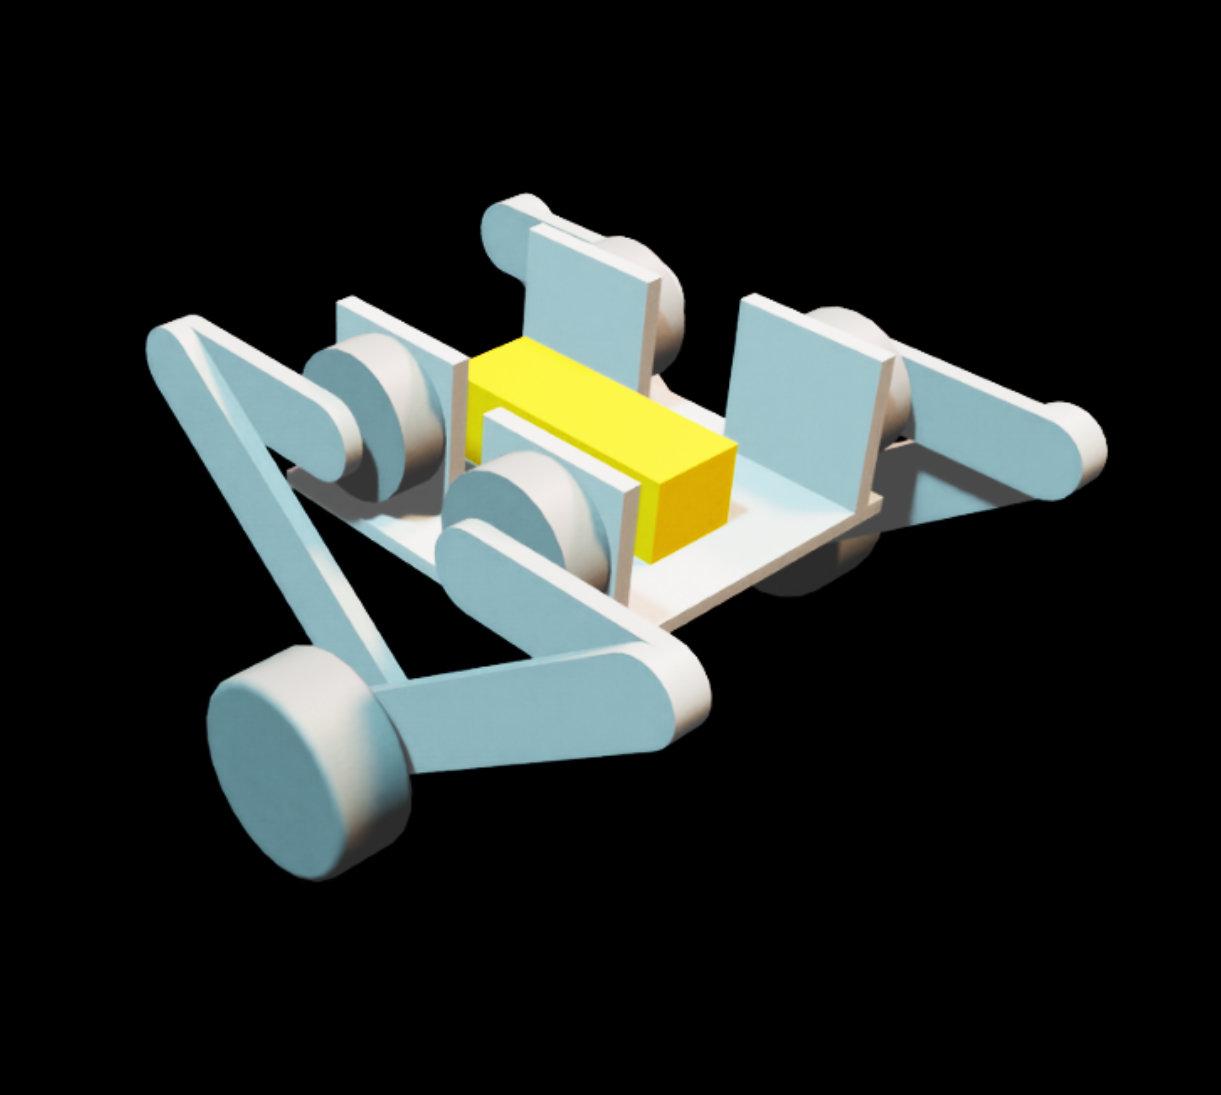
\includegraphics[width=4.00cm]{Images/Robot.png}};
    \draw[white] (B) -- (C);
    \draw[white] (D) -- (E);
    \node[below, text=white, font=\normalfont] at (F) {M3};
    \node[below, text=white, font=\normalfont] at (C) {M1};
    \node[above, text=white, font=\normalfont] at (E) {M2};
    \node[above, text=white, font=\normalfont] at (G) {M5};
    \node[above] at (H) {$x$};
    \node[above] at (H) {$x$};
    \draw[white] (H) -- (I);
    \node[above, text=white, font=\normalfont] at (I) {M4};
    \draw[white] (J) -- (K);
    \node[below, text=white, font=\normalfont] at (K) {M6};
    \draw[white] (L) -- (F);
  \end{tikzpicture}
\caption{USDC model robotske platforme z označenimi motorji M1--M6.}
\label{robot} 

\end{figure} 

%Kolesno-nožni roboti združujejo hitrost in agilnost z učin\-ko\-vi\-to\-stjo vožnje ter gibljivostjo nog, kar predstavlja že\-lje\-no kombinacijo sposobnosti robota v nestrokturiranih okoljih \cite{Liu2024Deve,Wang2025Whee}. Posebej zanimivi so dvokolesni roboti, ki delujejo po načelu inverznega nihala, zaradi česar pa so inherentno nestabilni. S tem se soočijo z enim izmed glavnih problemov sodobne mobilne robotike, v kateri je vedno popularnejša humanoidna robotika \cite{Bao2025Deep}. V članku \cite{Tofant2025Dife} so problem regulacije naklona dvokolesnega robota rešili s pomočjo notranje in zunanje zanke kaskadnega regulatorja, kjer notranja zanka uporablja kvadratični integralni regulator (angl. Linear Quadratic Integral controller, LQI), ki se je izkazal kot robustna rešitev vodenja robota v različnih okoljih. Razčlenitev njihovega regulatorja na dve regulaciji, za vsako kolo posebej, pa odpre vrzel v problemu, ki ga obravnavamo v tem delu; to je regulacija dvokolesnega robota, tako da stoji le na enem kolesu. Gre za nestabilen, sklopljen regulacijski problem: naklon je mogoče uravnavati le s pomočjo pogonskega kolesa, bočni nagib pa le s sklepi noge, pri čemer ravnovesna lega ni pokončna, temveč nagnjena.
  
  %Rešujemo  ga z globokim spodbujevalnim učenjem v simulaciji. Namesto da bi ravnovesni kot predpisali, funkcijo nagrajevanja zasnujemo tako, da ga politika med učenjem poišče sama; območje začetnih pogojev postopoma širimo s samodejnim kurikulumom, prenos iz simulacije na realni sistem pa dosežemo z randomizacijo domene, prilagojeno lastnostim dejanske strojne opreme. Rešitev je zasnovana tako, da se izvaja neposredno na vgrajenem mikrokrmilniku robota.
  %V našem primeru imamo tako zraven dinamike naklona še sklopljenost dinamike po nagibu, medtem ko imamo le eno stično točko, kar s klasičnim modelom \cite{Tofant2025Dife} težko opišemo, izpeljava analitičnega modela za tako lego pa je zahtevna. Avtorji v prispevku \cite{Tofant2025Dife} izrecno navajajo, da je uporaba strojnega učenja smiselna za nadaljnje delo. V našem primeru pa smo regulator nadgradili z uporabo pristopa spodbujevanega učenja (angl. reinforcement learning, RL), kjer se regulator uči na podlagi mnogih poskusov lovljenja ravnotežja v simulacijskem okolju, brez eksplicitno nastavljenega modela sklopljene dinamike \cite{Bao2025Deep}. Namesto da bi ravnovesni kot predpisali, funkcijo nagrajevanja zasnujemo tako, da ga politika med uče\-njem poišče sama, saj območje začetnih pogojev postopoma širimo z večfaznim učenjem. S tem se regulator nauči strategije (angl. policy), ki je robustna na celotno porazdelitev fizikalnih parametrov, upoštevajoč randomizacije domene (angl. domain randomization) prilagojeno lastnostim dejanske strojne opreme, kar omogoči uporabo strategije na realnem robotskem sistemu. 

%2. poglavje
\section{Robot in formulacija problema}
Platforma iz \cite{Tofant2025Dife} uporablja štiri motorje Xiaomi CyberGear (M1, M2, M4, M5) za gibljiv trup (nagib in višina), dva motorja DDSM115 (M3, M6) za pogon koles in stabilizacijo naklona, IMU BNO080 za orientacijo, baterijo ter mikrokrmilnik STM-32F446RE, na katerem teče regulacija (slika \ref{robot}).
  
  Motorji CyberGear so pozicijsko vodeni z impedančno regulacijo, kolesa DDSM115 pa tokovno oziroma navorno. Na podlagi dejanske platforme je bil ustvarjen poenostavljen 3D model v USDC (angl. USD Crate) formatu (slika \ref{robot}). 3D model smo uvozili v IsaacLab \cite{Mittal2025Isaa}, ki poleg geometrije opisuje tudi sklepe, pogone ter masne in vztrajnostne lastnosti povezanih teles. 
  
Glavni problem, ki ga je moral robot rešiti, je bilo ohranjanje bočno nagnjene nestabilne pozicije na enem kolesu z aktuatorji, krmiljenimi z nevronsko mrežo.
  
  V našem problemu smo robotu določili dva glavna kota: nagib $\varphi$ (angl. roll) (slika \ref{nakgib}) in naklon $\theta$ (angl. pitch) (slika \ref{naklon}). Nagib poteka okrog vzdolžne osi (vstran), medtem ko naklon poteka okrog prečne osi (naprej–nazaj).
 
Robot je bil v simulaciji postavljen na eno nogo, tako da je bilo le eno kolo v stiku s tlemi (M3), desna (zgornja) sklepa (M4, M5) sta v pokrčeni legi ($ 0^\circ $), leva (spodnja) sklepa (M1, M2) pa v iztegnjeni legi $ 45^\circ $. Zložitev zgornjih in izteg spodnjih sklepov premakne težišče in omogoči stabilnost na enem kolesu, zato so zgornje noge čim bolj zložene, spodnje pa le toliko odmaknjene, da jih lahko še normalno krmilimo v obe smeri. V tej postavitvi mora regulator hkrati vzdrževati dve sklopljeni veličini. Naklon uravnava prek toka edinega talnega kolesa (M3), bočni nagib pa prek kotov vseh sklepov (M1, M2, M4, M5). Ker pa nima nobene avtoritete okoli navpične osi, je  število neodvisnih krmilnih veličin manjše od števila prostostnih stopenj, zato je sistem pod\-aktuiran. Ravnovesna lega določena z geometrijo oziroma lego težišča, je bila predvidena v nagibu $ 47^\circ $, a je nismo predpisali, temveč jo je moral regulator vzdrževati sam. 
  
\begin{figure}[htbp]
\centering

  % Leva podslika (zaseda 45 % širine strani)
  \begin{subfigure}[b]{0.2\textwidth}
    \centering
    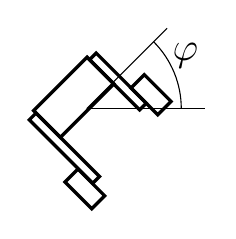
\begin{tikzpicture}[scale=0.24]
      \coordinate (A) at (-0.50, 1.25);
      \coordinate (D) at (5.75, 1.25);
      \coordinate (B) at (3.75, 5.50);
      \coordinate (C) at (4.72, 2.87);
      \draw[very thick, rotate around={-315.0:(-1.19,1.85)}] (-3.19,0.85) rectangle (0.81,2.85);
      \draw[very thick, rotate around={-315.0:(-1.68,-0.85)}] (-1.93,-3.22) rectangle (-1.43,1.53);
      \draw[very thick, rotate around={-315.0:(1.15,2.68)}] (0.9,0.81) rectangle (1.4,4.56);
      \draw[very thick, rotate around={-315.0:(-0.60,-3.00)}] (-1.09,-4) rectangle (-0.12,-2);
      \draw[very thick, rotate around={-315.0:(2.90,1.98)}] (2.4,0.98) rectangle (3.4,2.98);
      \draw (A) -- (D);
      \draw (A) -- (B);
      \draw (4.50, 1.25) arc (0.0:45.0:5.00);
      \node[above, font=\Large] at (C) {$\varphi$};
    \end{tikzpicture}
    \caption{}
    \label{nakgib}
  \end{subfigure}
  \hfill % Potisne desno sliko na rob
  % Desna podslika (zaseda 45 % širine strani)
  \begin{subfigure}[b]{0.2\textwidth}
    \centering
    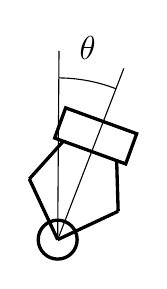
\begin{tikzpicture}[scale=0.24]
      \coordinate (B) at (-2.33, 0.36);
      \coordinate (C) at (-0.83, -2.85);
      \coordinate (D) at (2.29, 1.34);
      \coordinate (E) at (2.37, -1.35);
      \coordinate (F) at (-0.83, -2.85);
      \coordinate (A_1) at (-0.53, 2.36);
      \coordinate (G) at (-0.76, 7.14);
      \coordinate (H) at (0.75, 6.14);
      \coordinate (A_3) at (2.67, 6.21);
      \draw[very thick, rotate around={-20.0:(1.18,2.64)}] (-0.82,1.79) rectangle (3.18,3.49);
      \draw[very thick] (A_1) -- (B);
      \draw[very thick] (B) -- (C);
      \draw[very thick] (D) -- (E);
      \draw[very thick] (E) -- (C);
      \draw[very thick] (C) circle (1.03);
      \draw (C) -- (A_3);
      \draw (C) -- (G);
      \draw (2.24, 5.14) arc (69.0:89.5:8.56);
      \node[above, font=\large] at (H) {$\theta$};
    \end{tikzpicture}
    \caption{}
    \label{naklon}
  \end{subfigure}

\caption{(a) Kot nagiba, (b) Kot naklona}
\end{figure}

  %Če bi imeli samodejni prehod
%Robot je bil v začetnku simulacije postavljen na obe kolesi, iz koder se je samodejno prevrgel v pozicijo, da je bilo v stiku s tlemi le eno kolo (M3). Sklepe trupa (M1, M2, M4, M5) je imel v začetni legi $ 45^\circ $, ki jih je nato krmilil v razponu $ \pm 15^\circ $. Pozicija sklepov $ 45^\circ $ omogola, da jih lahke robot prosto krmili enakomerno v obe smeri. V tej postavitvi mora regulator hkrati vzdrževati dve sklopljeni veličini. Naklon uravnava prek toka edinega talnega kolesa, bočni nagib pa prek kotov sklepov. Ker pa nima nobene avtoritete okoli navpične osi, je  število neodvisnih krmilnih veličin manjše od števila prostostnih stopenj, zato je sistem pod\-aktuiran. Ravnovesna lega določena z geometrijo oziroma lego težišča, je bila predvidena v nagibu $ 47^\circ $, a je nismo predpisali, temveč jo je moral regulator vzdrževati sam.

%3. Ppoglavje
\section{Učno okolje in zasnova regulatorja}

  \begin{figure*}[t]
\begin{equation}
  R = 1.0\cdot p - 5.0\cdot\theta^2 - 0.3\cdot \Delta\theta^2 - 2\cdot \Delta \varphi^2 - 0.4\cdot v^2 - 0.15\cdot x^2 - 0.1\cdot j_{l+d} - 2.0\cdot fj_{l+d} - 0.003\cdot A_{M3} - 100\cdot e \label{nagrada enacba}
\end{equation}
\end{figure*}
Delno opazljiv markovski problem robota se izvaja v na\-črt\-no nepredvidljivem okolju v simulaciji in realnosti kar pomeni, da na robota vplivajo nepredvideni parametri kot so trenje, šum, zakasnitev senzorjev, itd. Za lažje naslavljanje tega izziva smo za arhitekturo nevronske mreže izbrali nevronsko mrežo s povratno zanko (angl. RNN, recurrent neural network), z uporabo pomnilnih celic GRU. Celica GRU skozi skrito stanje kodira časovno dinamiko sistema, kar robotu omogoča sprotno kompenzacijo fizikalnih netočnosti brez ročno nastavljenih filtrov ali zgodovinskih podatkov. GRU tako deluje kot ucljiv, nelinearni filter, ki bistveno poveča robustnost zaprto-zančnega vodenja.
  Učenje nevronske mreže je potekalo z algoritmom proksimalne optimizacije strategije (angl. PPO, proximal policy optimization) v fizikalni simulaciji s korakom 1 ms, na 4000 vzporednih okoljih na enem GPU-ju, z adaptivno hitrostjo učenja in 64 koraki med posodobitvami uteži.
  
  %Med hiperparametri algoritma PPO smo uporabili stopnjo učenja (angl.\ learning rate) $3 \times 10^{-4}$ z adaptivnim urnikom, ciljno divergenco KL (angl.\ Kullback--Leibler divergence) $0{,}01$, obrezovalni parameter (angl.\ clip parameter) $0{,}2$, koeficient entropije (angl.\ entropy coefficient) $0{.}005$, koeficient izgube vrednosti (angl.\ value loss coefficient) $1{,}0$, 4 učne epohe (angl.\ epochs), 4 mini-pakete (angl.\ mini-batches), omejitev norme gradienta (angl.\ max gradient norm) $0{,}5$ in začetni šum akcij (angl.\ action noise) s standardnim odklonom $0{,}2$.
  
  Agent prejme 6-razsežni vektor stanj (slika \ref{nevronska mreža}), jih procesira skozi prvi skriti sloj z 32 GRU celicami, nato pa čez 2 skrita sloja MLP z 32 nevroni in ReLU aktivacijsko funkcijo ter kot izhod vrne 5-razsežni vektor, ki je uporabljen kot vhod na treh motorjih robota. Prva komponenta izhodnega vektorja s pomočjo funkcije tanh določa tok talnega kolesa (DDSM115, M3), naslednji dve ciljni kot sprednjega in zadnjega levega sklepa (CyberGear M1 in M2) in zadnji dve ciljni kot sprednjega in zadnjega desnega sklepa (CyberGear M4 in M5). Dvignjeno kolo (M6) toka ne prejema, zato v akcijskem vektorju ne nastopi. Vsa opazovana stanja so normirana s fiksnimi, vnaprej določenimi vrednostmi, kar omogoča, da je aritmetika pri poznejši izvedbi na mikrokrmilniku identična simulacijski. 

Nagrada za učenje nevronske mreže je zasnovana na podlagi nepoznanosti dejanskih kotov nagiba v ravnovesni legi, zato v nagradi ne predpišemo željenega kota nagiba, temveč kaznujemo kvadrat njegove kotne hitrosti, kar omogoči, da ravnovesno lego nevronska mreža odkrije sama. Ker smo naklon ravnovesne lege poznali vnaprej ($ 0^\circ $), smo poleg kotne hitrosti kaznovali tudi po kotu samem. Nagrada ne vsebuje le opisanih členov, temveč tudi konstantno nagrado za preživetje, kazni za hitrost premika, velikost in gladkost sklepnih ukazov, porabo toka, ob predčasni prekinitvi pa enkratno kazen $-100$ (tabela \ref{tabela}, enačba \ref{nagrada enacba}). 
 
  Učenje strategije je potekalo 1300 iteracij, pri čemer se je razpon začetne perturbacije bočnega nagiba postopoma spreminjal skozi tri faze. Prva faza ($ \pm 5^\circ $) je trajala 350 iteracij, druga faza ($ \pm 8^\circ $) 350 iteracij in zadnja faza ($ \pm 11^\circ $) 600 iteracij. Z večfaznim učenjem se robot nauči spoprijemanja z drugimi koti ob začetku delovanja strategije, kar izboljša njeno robustnost.

  Trajanje epizode smo omejili z mejnimi vrednostmi treh spremenljivk. Epizoda se je zaključila, ko je bila absolutna vrednost naklona robota pet zaporednih korakov nad $ 40^\circ $ ali nagib robota pod $ 20^\circ $ ali nad $ 72^\circ $. Izpolnitev enega izmed teh pogojev je klasificirano kot padec. Če je robot uspešno ohranil naklon in nagib znotraj omejenih vrednosti, se je epizoda terminirala po 10 s. Tako vsaka epizoda pri frekvenci regulacije 50 Hz obsega maksimalno 500 regulacijskih korakov.

\begin{table}[h]
\caption{Členi nagrajevanja agenta.} \label{tabela}
\smallskip
\begin{center}
  \begin{tabular}{ | r | c | }
  \hline  
  \textbf{Nagrada/Kazen} & \textbf{Utež} \\ 
  \hline  
  Preživetje & $ +1.0 \cdot p $ \\
  Naklon & $ -5.0 \cdot \theta ^ 2 $ \\
  Sprememba naklona & $ -0.3 \cdot \Delta\theta ^ 2 $ \\
  Ukaz sklepov (L/D) & $-0.1 \cdot j_{l+d}$ \\
  Hitra sprememba sklepov (L/D) & $-2.0 \cdot fj_{l+d}$ \\
  Tok koles & $-0.003 \cdot A_{M3} $ \\
  Predčasna prekinitev & $-100 \cdot e$ \\
  Linearna hitrost & $ -0.4 \cdot v ^2 $ \\
  Pozicija & $ -0.15 \cdot x ^ 2 $ \\  
  Sprememba nagiba & $ -2 \cdot \Delta\varphi ^ 2 $ \\
  \hline  
  \end{tabular}
\end{center}
\end{table}


  % \begin{table}[h]
% \caption{Členi nagrajevanja agenta.} \label{tabela}
% \smallskip
% \begin{center}
%   \begin{tabular}{ | r | c | }
%   \hline  
%   \textbf{Nagrada/Kazen} & \textbf{Utež} \\ 
%   \hline  
%   Preživetje & $ +1.0 \cdot p $ \\
%   Naklon & $ -5.0 \cdot \theta ^ 2 $ \\
%   Sprememba naklona & $ -0.3 \cdot \Delta\theta ^ 2 $ \\
%   Ukaz levih sklepov & $-0.1 \cdot j_l$ \\
%   Ukaz desnih sklepov & $-0.1 \cdot j_d$ \\
%   \makecell[r]{Hitra sprememba\\levih sklepov} & $-2.0 \cdot fj_l$ \\
%   \makecell[r]{Hitra sprememba\\desnih sklepov} & $-2.0 \cdot fj_d$ \\
%   Tok koles & $-0.003 \cdot A_{M3} $ \\
%   Predčasna prekinitev & $-100 \cdot e$ \\
%   Linearna hitrost & $ -0.4 \cdot v ^2 $ \\
%   Pozicija & $ -0.15 \cdot x ^ 2 $ \\  
%   Sprememba nagiba & $ -2 \cdot \Delta\varphi ^ 2 $ \\
%   \hline  
%   \end{tabular}
% \end{center}
% \end{table}

%Od tu dalje je če imamo dve fazi epizode (odriv plus stabilizacija) -------------------------------------------------------
  
  %Ker je problem sestavljen iz dveh faz (odriv in stabilizacija), je nagrada prav tako razdeljena na dve enačbi. V prvi fazi epizode je nagrada $ R_1 $ usmerjena k stabilnemu odrivu robota proti nagibu $ 47^\circ $. Nagrada druge faze $ R_2 $ je zasnovana na podlagi nepoznanosti dejanskega stabilnega kota nagiba v ravnovesni legi, zato v nagradi ne predpišemo željenega kota nagiba, temveč kaznujemo kvadrat njegove kotne hitrosti, kar omogoči, da ravnovesno lego nevronska mreža odkrije sama. Ker smo naklon ravnovesne lege poznali vnaprej ($ 0^\circ $), smo poleg kotne hitrosti kaznovali tudi po kotu samem. Nagrada ne vsebuje le opisanih členov, temveč tudi konstantno nagrado za preživetje, kazni za hitrost premika, velikost in gladkost sklepnih ukazov, porabo toka, ob predčasni prekinitvi pa enkratno kazen $-100$ (tabela \ref{tab1}). 
  
% \begin{table}[h]
% \caption{Osnovni slogi pri oblikovanju prispevka.} \label{tab1}
% \smallskip
% \begin{center}
%   \begin{tabular}{ | r | c | c | }
%   \hline  
%   \textbf{Nagrada/Kazen} & \textbf{Utež} & \textbf{Faza}\\ 
%   \hline  
%   Preživetje & $ +1.0 \cdot p $ & \multirow{7}{*}{Obe}\\
%   Naklon & $ -5.0 \cdot \theta ^ 2 $   & \\
%   Sprememba naklona & $ -0.3 \cdot \Delta\theta ^ 2 $ & \\
%   Ukaz leveih sklepov & $-0.1 \cdot j_l$   & \\
%   \makecell[r]{Hitra sprememba\\levih sklepov} & $-2.0 \cdot fj_l$  & \\
%   Tok koles & $-0.003 \cdot A_{M3} $  & \\
%   Predčasna prekinitev & $-100 \cdot e$ & \\ \hline
%   Doseg odriva & $ -2 \cdot (\varphi - 47 ^ \circ)^ 2 $ & Faza 1 \\ \hline
%   Linearna hitrost & $ -0.4 \cdot v ^2 $ & \multirow {3}{*}{Faza 2}\\
%   Pozicija & $ -0.15 \cdot x ^ 2 $ & \\  
%   Sprememba nagiba & $ -2 \cdot \Delta\varphi ^ 2 $ & \\
%   Ukaz desnih sklepov & $-0.1 \cdot j_d$   & \\
%   \makecell[r]{Hitra sprememba\\desnih sklepov} & $-2.0 \cdot fj_d$  & \\
%   \hline  
%   \end{tabular}
% \end{center}
% \end{table}

%   \begin{strip}
% \begin{equation}
% R_1 = 1.0 \cdot p -5.0 \cdot \theta ^ 2 -0.3 \cdot \Delta \theta ^ 2 -0.1 \cdot j_l -2.0 \cdot fj_l -0.003 \cdot A_{M3} -100 \cdot e -2 \cdot (\varphi - 47 ^ \circ)^ 2
% \end{equation}
% \begin{equation}
%   R_2 =1.0\cdot p-5.0\cdot\theta^2-0.3\cdot \Delta  \theta ^2 -2\cdot \Delta \varphi^2-0.4\cdot v^2  -0.15\cdot x^2-0.1\cdot j_{l+d}-2.0\cdot fj_{l+d}-0.003\cdot A_{M3} -100\cdot e 
% \end{equation}
% \end{strip}

  %Trajanje epizode je bilo omejeno časovno in tudi glede na to ali je robot padel; naklon $ |\theta| > 40 ^ \circ$ ali nagib $ \varphi > 72 ^ \circ$ ali $ \varphi < 20 ^ \circ$, s tem da v prvi fazi upoštevamo le padec po naklonu. Ker smo želeli usmeriti robota v odriv v pravo smer smo poleg kazni se dodali terminacijo, ko se je odrinil v napačno smer; nagib $ \varphi < 15 ^ \circ$ Če je robot uspešno ohranil naklon in nagib znotraj omejenih vrednosti, se je epizoda terminirala po 10 s. Tako vsaka epizoda pri frekvenci regulacije 50 Hz obsega maksimalno 500 regulacijskih korakov.

% -------------------------------------------------------

  
%  Nagrada za učenje nevronske mreže je zasnovana na podlagi nepoznanosti dejanskih kotov nagiba v ravnovesni legi, zato v nagradi ne predpišemo željenega kota nagiba, temveč kaznujemo kvadrat njegove kotne hitrosti, kar omogoči, da ravnovesno lego nevronska mreža odkrije sama. Ker smo naklon ravnovesne lege poznali vnaprej ($ 0^\circ $), smo poleg kotne hitrosti kaznovali tudi po kotu samem. Nagrada ne vsebuje le opisanih členov, temveč tudi konstantno nagrado za preživetje, kazni za hitrost premika, velikost in gladkost sklepnih ukazov, porabo toka, ob predčasni prekinitvi pa enkratno kazen $-100$. 
%Večfazno učenje je potekalo 1500 iteracij, pri čemer se je razpon začetne perturbacije bočnega nagiba postopoma spreminjal skozi štiri faze. Prva faza ($ \pm 3^\circ $) je trajala 500 iteracij, druga faza ($ \pm 8^\circ $) 300 iteracij, tretja faza ($ \pm 15^\circ $) 300 iteracij in zadnja faza ($ \pm 20^\circ $) 400 iteracij. Z večfaznim učenjem se robot nauči spoprijemanja z drugimi koti začetka delovanja regulacije. 
%Trajanje epizode smo omejili z mejnimi vrednostmi treh spremenljivk. Epizoda se je zaključila, ko je bila absolutna vrednost naklona robota pet zaporednih korakov nad $ 40^\circ $ ali nagib robota pod $ 20^\circ $ ali nad $ 72^\circ $. Izpolnitev enega izmed teh pogojev je klasificirano kot padec. Če je robot uspešno ohranil naklon in nagib znotraj omejenih vrednosti, se je epizoda terminirala po 10 s. Tako vsaka epizoda pri frekvenci regulacije 50 Hz obsega maksimalno 500 regulacijskih korakov.
  

%Nevronska mreža
\begin{figure*}[t] 
\centering
\begin{tikzpicture}[
   scale=0.7,
    node distance=6mm,
    io/.style={circle, draw, minimum size=4.5mm, inner sep=0pt},
    hid/.style={rounded corners, draw, fill=black!4,
                minimum width=10mm, minimum height=34mm, align=center},
    norm/.style={rounded corners, draw, fill=black!8,
                 minimum width=6mm, minimum height=34mm, align=center},
    >=stealth
]

% --- vhodni sloj (12 nevronov) ---
\foreach \i in {1,...,6}
    \node[io] (in\i) at (0, {2.5 - \i*0.7}) {};
\node[left=2mm of in1] (lbl1) {\footnotesize nagib};
\node[left=2mm of in2] (lbl2) {\footnotesize kotna hitrost nagiba};
\node[left=2mm of in3] (lbl3) {\footnotesize naklon};
\node[left=2mm of in4] (lbl4) {\footnotesize kotna hitrost naklona};
\node[left=2mm of in5] (lbl5) {\footnotesize odmik po x osi};
\node[left=2mm of in6] (lbl6) {\footnotesize linearna hitrost};              

% --- normalizacija (fiksne konstante) ---
\node[norm] (nrm) at (1.5, 0.0) {\rotatebox{90}{\footnotesize normalizacija}};

% --- skrita sloja (bloka) ---
\node[hid] (h1) at (3.5, 0.00) {GRU \\ + \\MLP};

% --- izhodni sloj (3 nevroni) ---
\node[io] (out1) at (6, 1.8) {};
\node[io] (out2) at (6, 0.9) {};
\node[io] (out3) at (6, 0) {};
\node[io] (out4) at (6, -0.9) {};
\node[io] (out5) at (6, -1.8) {};
\node[right=2mm of out1] (lblo1) {\footnotesize kot motorja M1};
\node[right=2mm of out2] (lblo2) {\footnotesize kot motorja M2};
\node[right=2mm of out3] (lblo3) {\footnotesize tok motorja M3};
\node[right=2mm of out4] (lblo4) {\footnotesize kot motorja M4};
\node[right=2mm of out5] (lblo5) {\footnotesize kot motorja M5};

% --- normalizacija (fiksne konstante) ---
\node[norm] (nrm2) at (10.5, 0.00) {\rotatebox{90}{\footnotesize normalizacija}};

% --- slika simulacije
\node[inner sep=0pt] (simulation) at (13.8, 0) {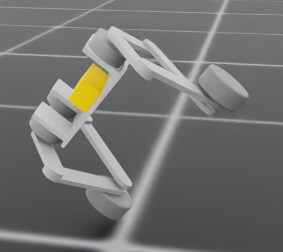
\includegraphics[width=.18\textwidth]{Images/Simulation.png}}; 
\node[above=1mm of simulation] {Simulacija};

% --- povezave ---
\foreach \i in {1,...,6}
    \draw[->, black!70] (in\i.east) -- (nrm.west |- in\i.east);
\draw[->, black!60] (nrm.east) -- (h1.west);
\foreach \o in {1,2,3,4,5}
    \draw[->, black!70] (h1.east) -- (out\o.west);;
\foreach \o in {1,2,3,4,5}
    \draw[->, black!70] (lblo\o.east) -- (nrm2.west |- out\o.east);

\draw[->, black!70] (nrm2.east) -- (simulation.west);
\draw[black!70] (simulation.south) |- (-4.5, -2.5) -- (-4.5, 1.8);

\foreach \i in {1,...,6}
    \draw[->, black!70] (-4.5, {2.5 - \i*0.7}) -- (lbl\i.west);

\draw[->, dashed, black, thick] (simulation.north west) -- ++(0,0.8) -| (h1.north) 
    node[pos=0.2, above] {Nagrada $R_{1,2}$};

\end{tikzpicture}
\caption{Arhitektura strategije: 6-razsežni vektor stanja se najprej normira
s fiksnimi konstantami, sledi obdelava z RNN nevronsko mrežo, normalizacija izhodnih veličin in simulacija. 
3 izhodne krmilne veličine.}
\label{nevronska mreža}
\end{figure*} 

%4. Ppoglavje
\section{Priprava za prenos v realno okolje}
Cilj tega prispevka ni simulacija sama po sebi ampak mož\-nost prenosljivosti predlagane rešitve na realni sistem. Največji problem delovanja Sim2Real (angl. sim-to-real) je nepopolnost realnega okolja in strojne opreme, kar ni vedno mogoče doseči z virtualnim modelom. To rešimo z integracijo rekurzivne arhitekture GRU in strogim upo\-šte\-va\-njem omejitev strojne opreme. Upoštevali smo velikost pomnilnika mikrokrmilnika STM32F446RE, zaradi česar smo nevronsko mrežo omejili na le tri skrite sloje z 32 nevroni oz. GRU celicami (slika \ref{nevronska mreža}). Nevronska mreža s skritim slojem 32 GRU celic in dvema skritima slojema po 32 nevronov vsebuje približno 6600 parametrov, kar v 32-bitnem zapisu s plavajočo vejico znaša okoli 26 kB. To predstavlja zanemarljiv delež pomnilnika mikrokrmilnika STM32F446RE (512 kB bliskovnega pomnilnika in 128 kB SRAM), rezultati sklepanja pa zahtevajo manj kot 1 kB delovnega pomnilnika. En prehod skozi mrežo obsega več tisoč množenj in seštevanj, kar na jedru Cortex-M4 traja nekaj $10\,\mu\text{s}$, kar je bistveno manj od regulacijskega koraka 20 ms. Za čim večjo računsko hitrost smo uporabili fiksno normalizacijo vhodov nevronske mreže s konstantami, za aktivacijsko funkcijo pa izbrali računsko nezahtevno funkcijo ReLU. Na realnem sistemu kontrolna zanka zaradi omejitev komunikacijskih vodil CAN in RS\-485 teče s frekvenco 50 Hz, zato smo regulacijo z nevronsko mrežo na enako frekvenco omejili tudi v simulaciji. Zaradi zaščite motorjev DDSM115 smo prav tako omejili izhod nevronske mreže za tok kolesa s funkcijo $\tanh$, ki tok zvezno preslika v območje $\pm 2{,}0$~A in tako prepreči preseganje varne tokovne meje.
  
  Sim2Real smo želeli izboljšati še z dodajanjem randomizacije domene (angl. domain randomization), pri čemer celice GRU skozi sprotno posodabljanje skritega stanja delujejo kot implicitni identifikator spreminjajočega se sistema. Namesto da bi poskušali parametre realne platforme natančno izmeriti in poustvariti v simulaciji, strategijo učimo na celotni porazdelitvi verjetnih vrednosti, s čimer predvidevamo, da je velika možnost, da realna platforma deluje z vrednostmi, ki padejo znotraj te porazdelitve. Izdelali smo funkcijo, ki na začetku vsake epizode vpelje randomizacijo domene in naključno spreminja ojačenje motorjev (od $0{,}8$ do $1{,}2$), prag prenehanja delovanja motorjev zaradi trenja (od $0{,}03$ do $0{,}20$~A), odmik toka zaradi nesimetrije motorja (od $-0{,}08$ do $0{,}08$~A), časovno konstanto tokovne zanke (od $0{,}005$ do $0{,}020$~s), tokovno omejitev posameznega motorja (od $1{,}6$ do $2{,}4$~A), odmik meritve naklona zaradi napake v montaži ali kalibraciji IMU senzorja (od $-0{,}5$ do $0{,}5$°) ter zakasnitev akcij na motorjih in zakasnitev opazovanj senzorjev (naključno $0$ ali $1$ korak). Prisotnost zakasnitev in nelinearnih šumov (Gaussov šum naklona s $\sigma = 0{,}15$° in kotne hitrosti s $\sigma = 0{,}02$~rad/s) v vsakem koraku simulacije dodatno utemeljuje uporabo arhitekture GRU, saj mreža s spominom uspešno kompenzira delno opazovanje stanja brez vnosa faznega zamika.
  
%5. Ppoglavje
\begin{figure*}[htbp]
    \centering
    
    % --- STOLPEC (a) ---
    \begin{subfigure}[b]{0.24\textwidth}
        \centering
        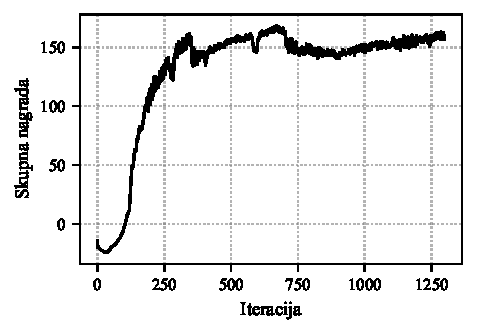
\includegraphics[width=\textwidth]{Images/Episode_reward.pdf}
        \caption{}
        \label{Nagrada}
    \end{subfigure}
    \hfill % Avtomatski vodoravni razmak med stolpci
  % --- STOLPEC (b) ---
    \begin{subfigure}[b]{0.24\textwidth}
        \centering
        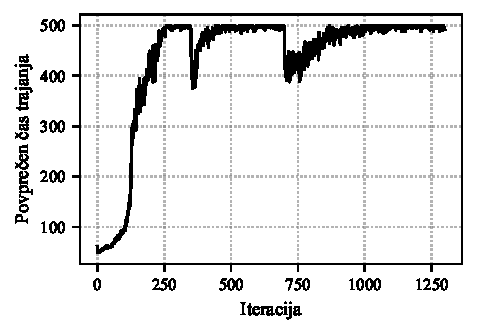
\includegraphics[width=\textwidth]{Images/Episode_length.pdf}
        \caption{}
        \label{Dolžina epizode}
    \end{subfigure}
    \hfill % Avtomatski vodoravni razmak med stolpci
  % --- STOLPEC (d) ---
    \begin{subfigure}[b]{0.24\textwidth}
        \centering
        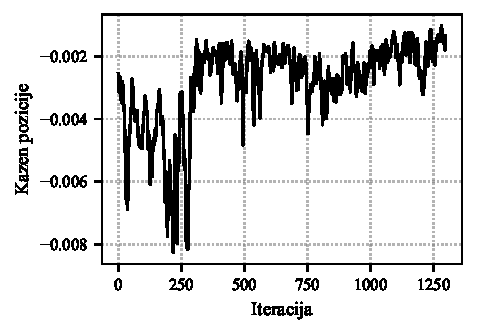
\includegraphics[width=\textwidth]{Images/Position_reward.pdf}
        \caption{}
        \label{Kazen pozicije}
    \end{subfigure}
    \hfill % Avtomatski vodoravni razmak med stolpci
    % --- STOLPEC (c) ---
    \begin{subfigure}[b]{0.24\textwidth}
        \centering
        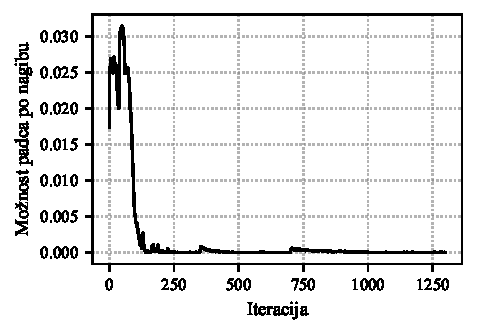
\includegraphics[width=\textwidth]{Images/Roll_fall_rate.pdf}
        \caption{}
        \label{Padec nagiba}
    \end{subfigure}
    \hfill % Avtomatski vodoravni razmak med stolpci
      % --- STOLPEC (c) ---
    \begin{subfigure}[b]{0.24\textwidth}
        \centering
        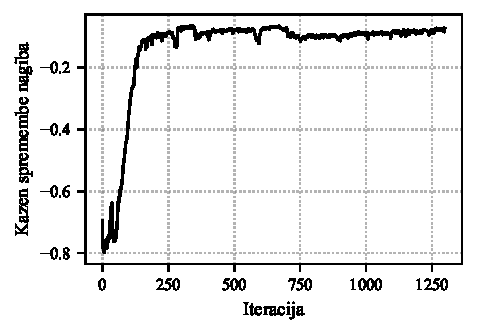
\includegraphics[width=\textwidth]{Images/Rollrate_penalty.pdf}
        \caption{}
        \label{Hitrost nagiba}
    \end{subfigure}
    \hfill % Avtomatski vodoravni razmak med stolpci
    % --- STOLPEC (c) ---
    \begin{subfigure}[b]{0.24\textwidth}
        \centering
        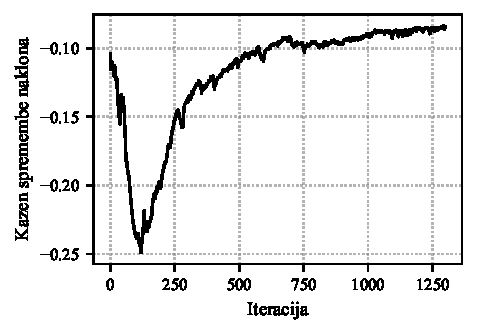
\includegraphics[width=\textwidth]{Images/Pitchrate_penalty.pdf}
        \caption{}
        \label{Hitrost naklona}
    \end{subfigure}
    \hfill % Avtomatski vodoravni razmak med stolpci
      % --- STOLPEC (c) ---
    \begin{subfigure}[b]{0.24\textwidth}
        \centering
        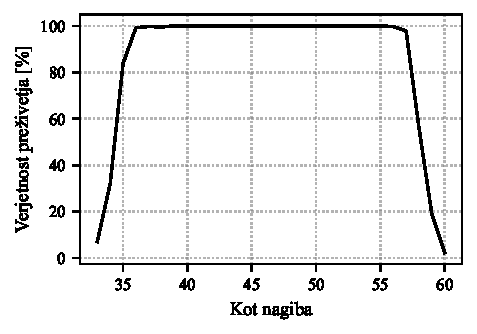
\includegraphics[width=\textwidth]{Images/survival_rate.pdf}
        \caption{}
        \label{Verjetnost preživetja}
    \end{subfigure}
    \hfill % Avtomatski vodoravni razmak med stolpci

    \caption{(a) Nagrada na epizodo, (b) Povprečen čas trajanja epizode, (c) Kazen pozicije na epizodo, (d) Možnost padca po nagiba v vsakem koraku, (e) Kazen spremembe kota nagiba, (f) Kazen spremembe kota naklona, (g) Verjetnost preživetja glede na začetni kot nagiba.}
    \label{fig:glavna_slika_6}
\end{figure*} 

\section{Eksperimentalni rezultati}
Posluževanje večfaznega učenja je očitno vidno predvsem v grafih \ref{Nagrada}, \ref{Dolžina epizode} in \ref{Padec nagiba} kot kratkotrajni padci skupne nagrade in povprečnega trajanja epizode ter rahlo povečanje verjetnosti padca, čemur sledi počasnejša konvergenca nazaj proti maksimumu z vsako težjo fazo. 
Graf \ref{Kazen pozicije} teh prehodov ne izkazuje jasno, kar nakazuje stabilnost sistema znotraj posamezne faze. Ker robot ravnotežje ohranja s sočasnim delovanjem vseh petih motorjev (M1–M5), se neprestano rahlo pomika naprej, nazaj, gor in dol, zaradi česar kazni v grafih \ref{Kazen pozicije}, \ref{Hitrost nagiba} in \ref{Hitrost naklona} konvergirajo proti majhni, a nikoli ničelni vrednosti — kar pomeni, da je robot ravnotežje našel in ga ohranjal znotraj majhnih odstopanj nagiba in naklona.

  Za testiranje delovanja smo ustvarili simulacijsko okolje, v katerega smo robota postavili pod različnimi koti nagiba ter opazovali kolikšna je verjetnost, da najde in ohrani ravnotežno lego do konca epizode trajajoče 10 s. S tem smo želeli simulirati prehod iz dvokolesnega ravnovesja v enokolesno ravnovesno lego. Za večjo robustnost sistema smo primerjali verjetnost preživetja v velikem razponu začetnega nagiba ob začetku delovanja strategije. Testiranje je potekalo v 64 okoljih, kjer smo za vsak kot nagiba vsako okolje opazovali 6 epizod. Glede na graf \ref{Verjetnost preživetja} je strategija najuspešnejša med $ 36^\circ $ in $ 57^\circ $, kjer dosega skoraj konstantno 100 \% verjetnost preživetja. Tukaj se vidi povezava med učenimi vrednostmi in uspešnostjo delovanja, saj je bila strategija učena na maksimalnem razponu $ 47^\circ \pm 11^\circ $, kjer tudi deluje najbolj robustno. Takoj ko pa začetni naklon pade izven mej učenja pa se lahko opazi strm padec verjetnosti preživetja.
  %Najvišja dosežena verjetnost preživetja znaša 100 \% pri nagibu  $ 47^\circ $. Ker je regulacija naj\-uspešnejša prav okrog napovedanih $47^\circ$, se potrdi, da je strategija ravnovesno lego odkrila sama, brez predpisanega referenčnega kota nagiba.
  
%6. Ppoglavje
\section{Zaključek}
V prispevku smo obravnavali ravnotežje kolesno-nožnega robota na enem samem kolesu, ki predstavlja nestabilen, sklopljen in podaktuiran regulacijski problem z nagnjeno ravnovesno lego, ki ga s klasičnim modelom težko opišemo. Pokazali smo, da je takšen problem mogoče regulirati s strategijo učeno z globokim spodbujevanim učenjem, ki uporablja celice GRU kot osnovno arhitekturo. Strategija se je v mejnem območju učenja (začetni nagib $47^\circ \pm 11^\circ$) izkazala zanesljivo. Ker je robustno območje delovanja tako veliko, je tudi prehod iz dvokolesnega v enokolesno ravnovesje lažje. Rešitev namenoma deluje v okviru omejitev ciljne strojne opreme z majhno mrežo, fiksno normalizacijo, frekvenco regulacije $50$ Hz ter z randomizacijo domene, prilagojeno naključnosti realnega okolja, kar odpira pot neposrednemu prenosu na vgrajeni sistem v realnem okolju. 

Nadaljevanje tega dela definitivno odpira vrata za uporabo takšnih robotskih sistemov v realnih nestrukturiranih območjih, kjer bi lahko s pomočjo podobnih inherentno nestabilnih gibov omogočilo mobilnim robotom boljše premagovanje ovir. Uporaba celic GRU bi tako lahko bila uporabljena za boljše napovedovanje naslednjih stanj in premagovanju nestabilnostih v okolju samem.



  
\small

% \bibliographystyle{IEEEtran} % Or 'ieeetr' for IEEE style
% \bibliography{bibliography.bib}  % 'references' matches the name of your .bib file 

\begin{thebibliography}{5}

\bibitem{Wang2025Whee}
K.~Wang \emph{et al.}, ``Wheeled-legged robots for multi-terrain
locomotion in plateau environments,'' \emph{Biomimetic Intelligence
and Robotics}, vol.~5, no.~3, p.~100256, 2025.

\bibitem{Rudin2022Lear}
N.~Rudin, D.~Hoeller, P.~Reist, and M.~Hutter, ``Learning to walk in
minutes using massively parallel deep reinforcement learning,''
\emph{arXiv preprint arXiv:2109.11978}, 2022.

\bibitem{Smirnov2025RLBe}
I.~Smirnov and S.~Gu, ``RLBenchNet: The right network for the right
reinforcement learning task,'' \emph{arXiv preprint
arXiv:2505.15040}, 2025.

\bibitem{Tofant2025Dife}
J.~Tofant and D.~Gleich, ``Diferenčno vodenje agilnega
dvokolesnega mobilnega robota,'' in \emph{Zbornik konference ERK
2025}, Portoro\v{z}, Slovenija, 2025, pp.~597--600.

\bibitem{Mittal2025Isaa}
M.~Mittal \emph{et al.}, ``Isaac Lab: A GPU-accelerated simulation
framework for multi-modal robot learning,'' \emph{arXiv preprint
arXiv:2511.04831}, 2025.

\end{thebibliography}
  
%\begin{thebibliography}{1}
%\bibitem{ERK} ERK, http://www.ieee.si/erk/index.html 
%\bibitem{Zbornik} B. Zajc, A. Trost: Zbornik triindvajsete mednarodne Elektrotehniške in računalniške konference ERK 2014, 22. - 24. %September 2014, Portorož, Slovenija

%\end{thebibliography}

\end{document}